\documentclass[10pt]{article}
\usepackage{../setup}
\vspace{-8ex}
\date{}

\graphicspath{ {./figs/} }
\newcommand{\figscalingfactor}{0.85}

\begin{document}

\title{\textbf{\Large{\textsc{ECE410:} Linear Control Systems}} \\ \Large{Output Feedback Stabilization of a Cart-Pendulum Robot} \\ \textbf{\small{PRA102}}\vspace{-0.3cm}}
\author{Pranshu Malik, Varun Sampat \\ \footnotesize{1004138916}, \footnotesize{1003859602}\vspace{-3cm}}

\maketitle

\section{Noiseless State Estimation}

\begin{equation*}
    L_1 = \begin{bmatrix}
    -22.9338 & -1.0388 \\
    -130.7798 & -14.0775 \\ 
    -0.9570 & -23.0662 \\ 
    -10.9830 & -168.2588
    \end{bmatrix}
\end{equation*}

\begin{equation*}
    L_2 = 10^{3} \times \begin{bmatrix}
    -0.0829  & -0.0011 \\
    -1.7161  & -0.0464 \\ 
    -0.0009  & -0.0831 \\ 
    -0.0380  & -1.7629
    \end{bmatrix}
\end{equation*}

\begin{figure}
    \centering
    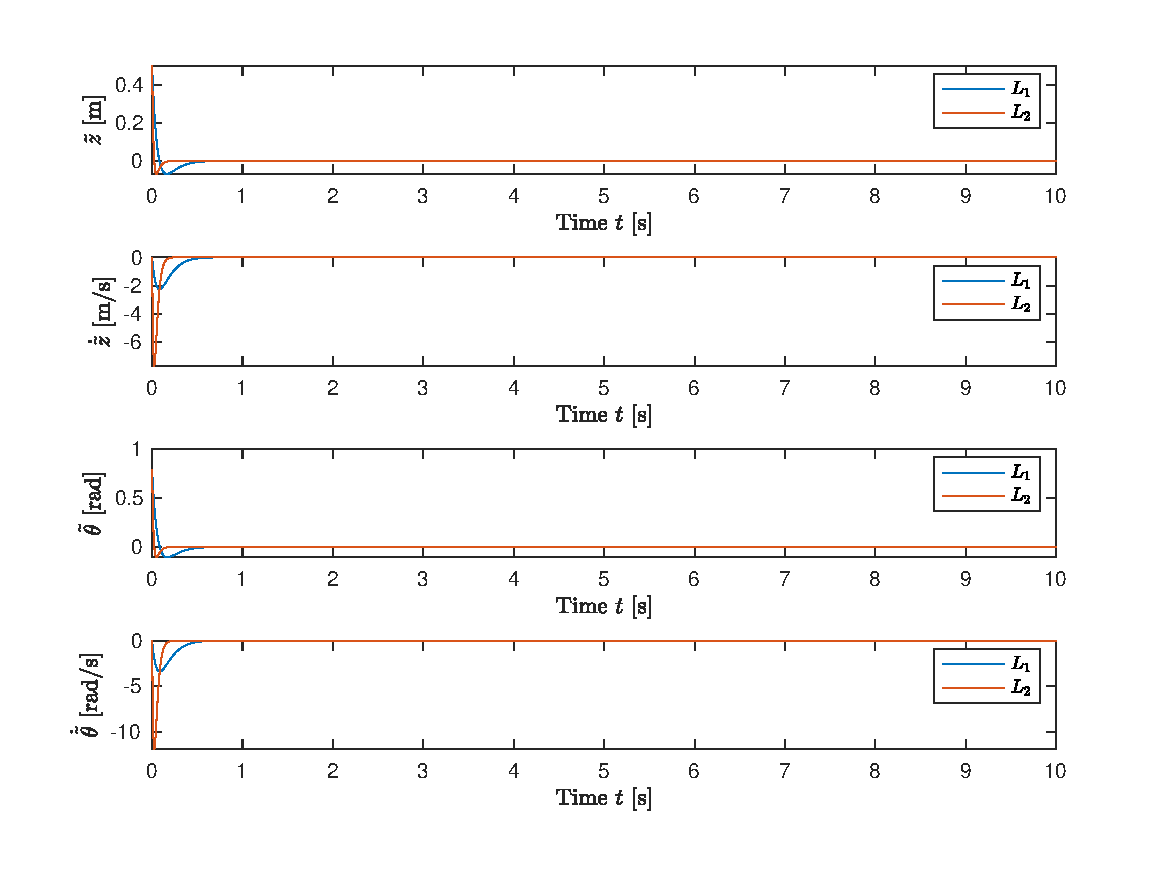
\includegraphics[\figscalingfactor\textwidth]{lab4/figs/lin_noiseless_state_est_error.pdf}
    \caption{Linear Noiseless State Estimation Error}
    \label{fig:lin_noiseless_state_est_error}
\end{figure}

\begin{figure}
    \centering
    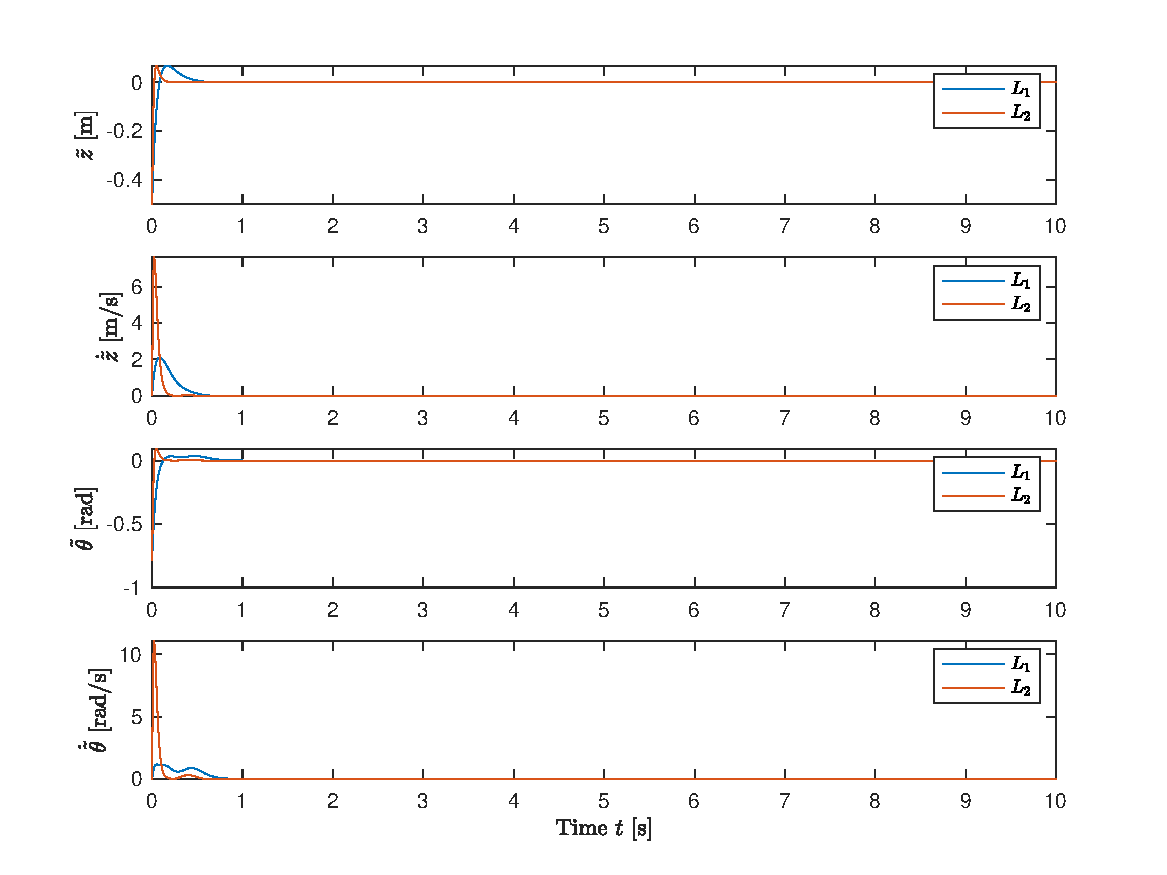
\includegraphics[\figscalingfactor\textwidth]{lab4/figs/nlin_noiseless_state_est_error.pdf}
    \caption{Nonlinear Noiseless State Estimation Error}
    \label{fig:nlin_noiseless_state_est_error}
\end{figure}

\section{State estimation with measurement noise}

\begin{figure}
    \centering
    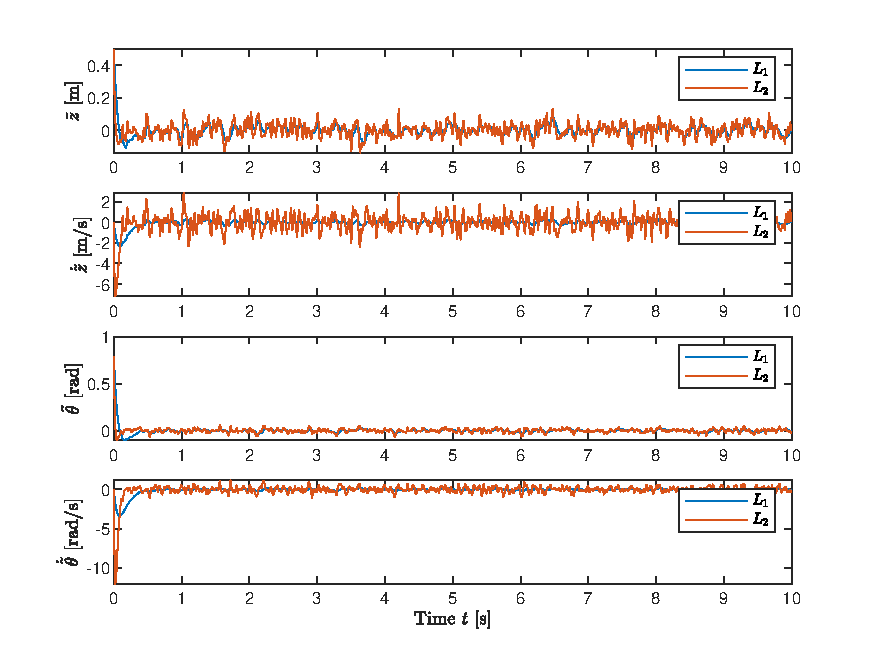
\includegraphics[\figscalingfactor\textwidth]{lab4/figs/lin_noisy_state_est_error.pdf}
    \caption{Linear Noisy State Estimation Error}
    \label{fig:lin_noisy_state_est_error}
\end{figure}

\section{Noiseless output feedback control} 

\begin{figure}
    \centering
    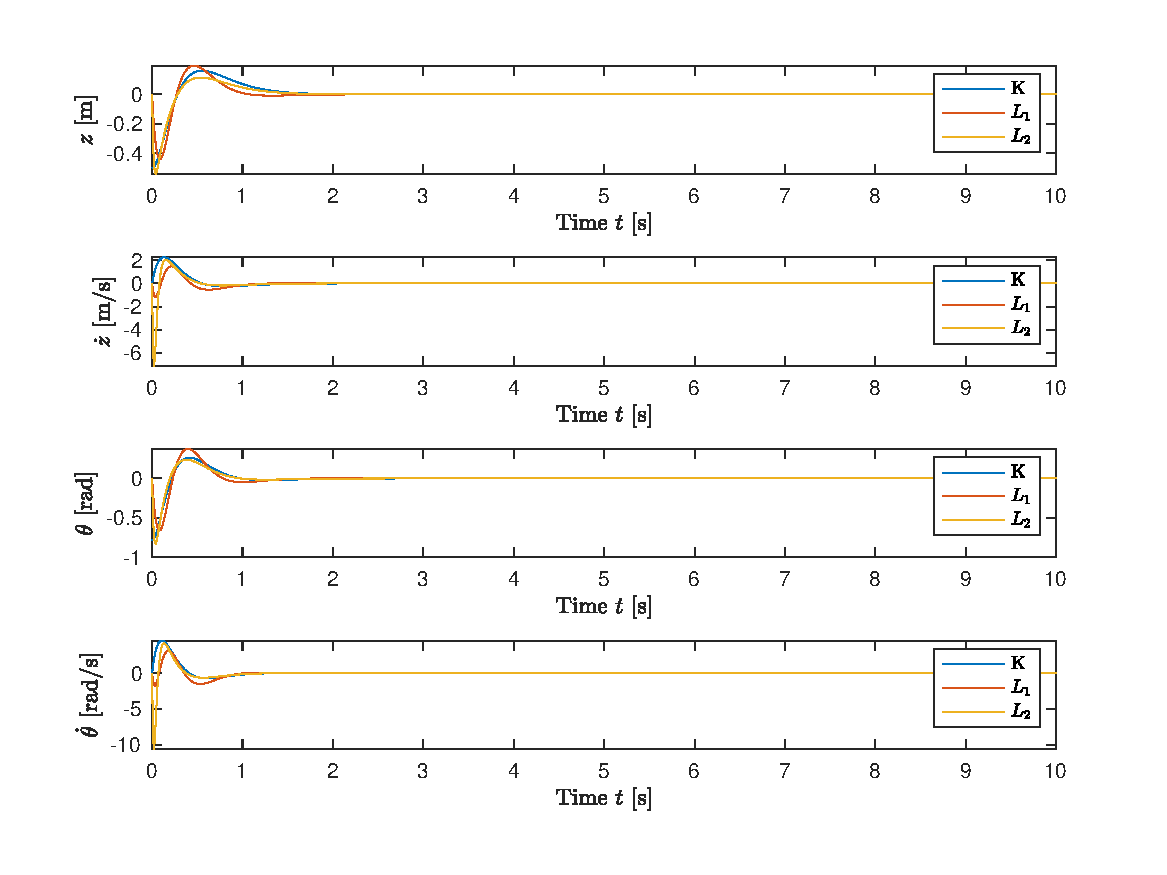
\includegraphics[\figscalingfactor\textwidth]{lab4/figs/lin_noiseless_state_est_error_feedback.pdf}
    \caption{Linear System State Evolution with feedback control}
    \label{fig:lin_noiseless_state_est_error_feedback}
\end{figure}


\begin{figure}
    \centering
    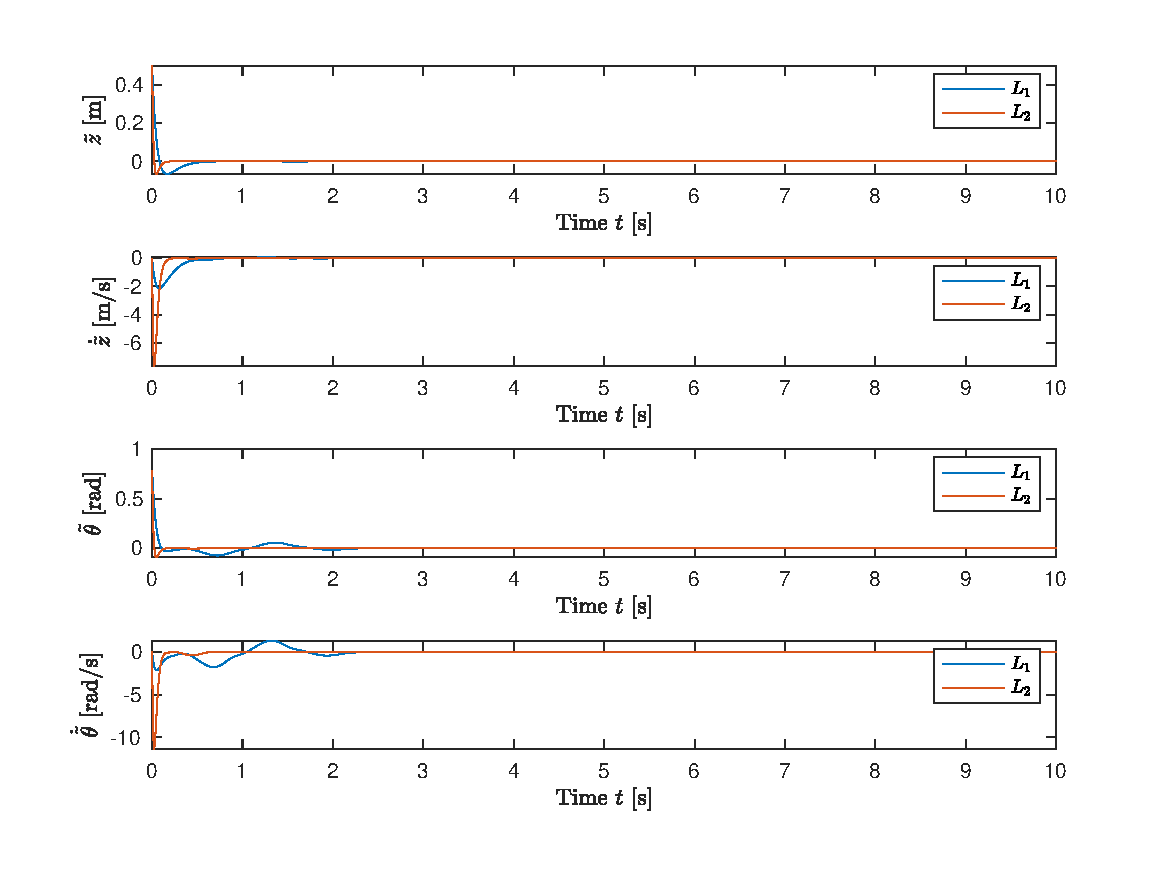
\includegraphics[\figscalingfactor\textwidth]{lab4/figs/nlin_noiseless_state_est_error_feedback.pdf}
    \caption{Nonlinear System State Evolution with feedback control}
    \label{fig:nlin_noiseless_state_est_error_feedback}
\end{figure}


\section{Output feedback control with measurement noise}

\begin{figure}
    \centering
    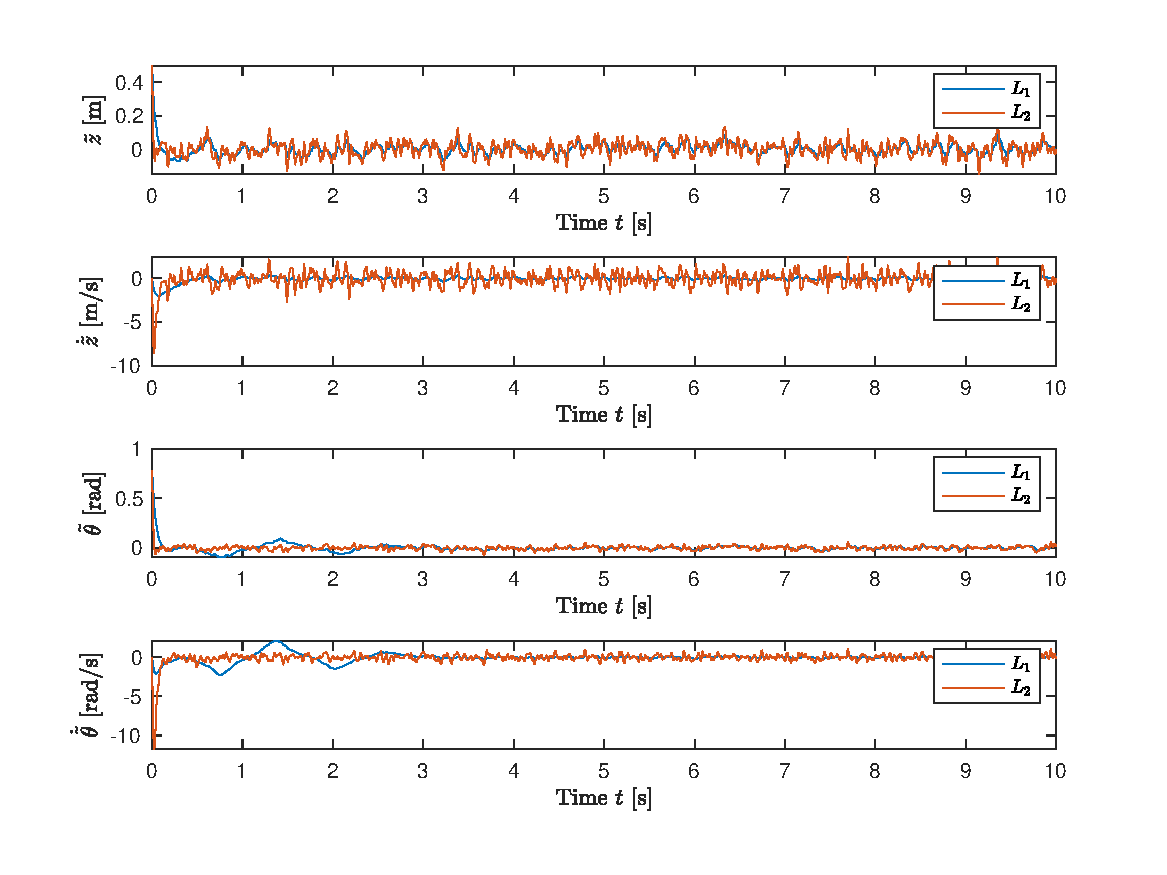
\includegraphics[\figscalingfactor\textwidth]{lab4/figs/nlin_noisy_state_est_error_feedback.pdf}
    \caption{Noisy Nonlinear System State Evolution with feedback control}
    \label{fig:nlin_noisy_state_est_error_feedback}
\end{figure}

\end{document}